% !TEX encoding = UTF-8 Unicode
\documentclass{standalone}
% \usepackage{pgfplots}
% \pgfplotsset{compat=1.11}

\renewcommand{\familydefault}{\sfdefault}
% \usepackage[version=0.96]{pgf}
\usepackage{tikz}
% \usetikzlibrary{arrows,shapes,automata,backgrounds,petri,positioning}
% \usetikzlibrary{decorations.pathmorphing}
% \usetikzlibrary{decorations.shapes}
% \usetikzlibrary{decorations.text}
% \usetikzlibrary{decorations.fractals}
% \usetikzlibrary{decorations.footprints}
% \usetikzlibrary{shadows}
% \usetikzlibrary{calc}
% \usetikzlibrary{spy}

% \pgfplotsset{compat=1.11}
\usepackage[utf8]{inputenc}
% \usepackage[vietnam]{babel}



%% ========= long bar notation ==============================
\makeatletter
\newsavebox\myboxA
\newsavebox\myboxB
\newlength\mylenA
\newcommand*\lbar[2][.75]{%
    \sbox{\myboxA}{$\m@th#2$}%
    \setbox\myboxB\null% Phantom box
    \ht\myboxB=\ht\myboxA%
    \dp\myboxB=\dp\myboxA%
    \wd\myboxB=#1\wd\myboxA% Scale phantom
    \sbox\myboxB{$\m@th\overline{\copy\myboxB}$}%  Overlined phantom
    \setlength\mylenA{\the\wd\myboxA}%   calc width diff
    \addtolength\mylenA{-\the\wd\myboxB}%
    \ifdim\wd\myboxB<\wd\myboxA%
       \rlap{\hskip 0.5\mylenA\usebox\myboxB}{\usebox\myboxA}%
    \else
        \hskip -0.3\mylenA\rlap{\usebox\myboxA}{\hskip 0.3\mylenA\usebox\myboxB}%
    \fi}
\makeatother

\def\lbD{\lbar{\bD}}
\def\lbY{\lbar{\mathb{Y}}}
\def\lbX{\lbar{\bX}}


\def\d{.9}
% \def\p{5.1}
\def\q{-.9}
% \def\sc{25}

\newcommand{\nn}[4]{
    \begin{scope}[xshift = #1*\d cm, yshift = #2*\q cm]
        
    \node at (0, 0) [anchor = east, draw, inner sep = 0, fill = #3!20, minimum height = .9cm, minimum width = .9cm] {#4};
    \end{scope}
}

\newcommand{\nnn}[4]{
    \begin{scope}[xshift = #1*\d cm, yshift = #2*\q cm]
        
    \node at (0, 0) [anchor = east, align = left,  draw, inner sep = 0, fill = #3!30, minimum height = .9cm, minimum width = .9cm] {#4};
    \end{scope}
}

\newcommand{\nb}[4]{
    \begin{scope}[xshift = #1*\d cm, yshift = #2*\q cm]
        
    \node at (0, 0) [anchor = east, align = left, inner sep = 0, fill = #3!30, minimum height = .6cm, minimum width = .6cm] {#4};
    \end{scope}
}

\begin{document}
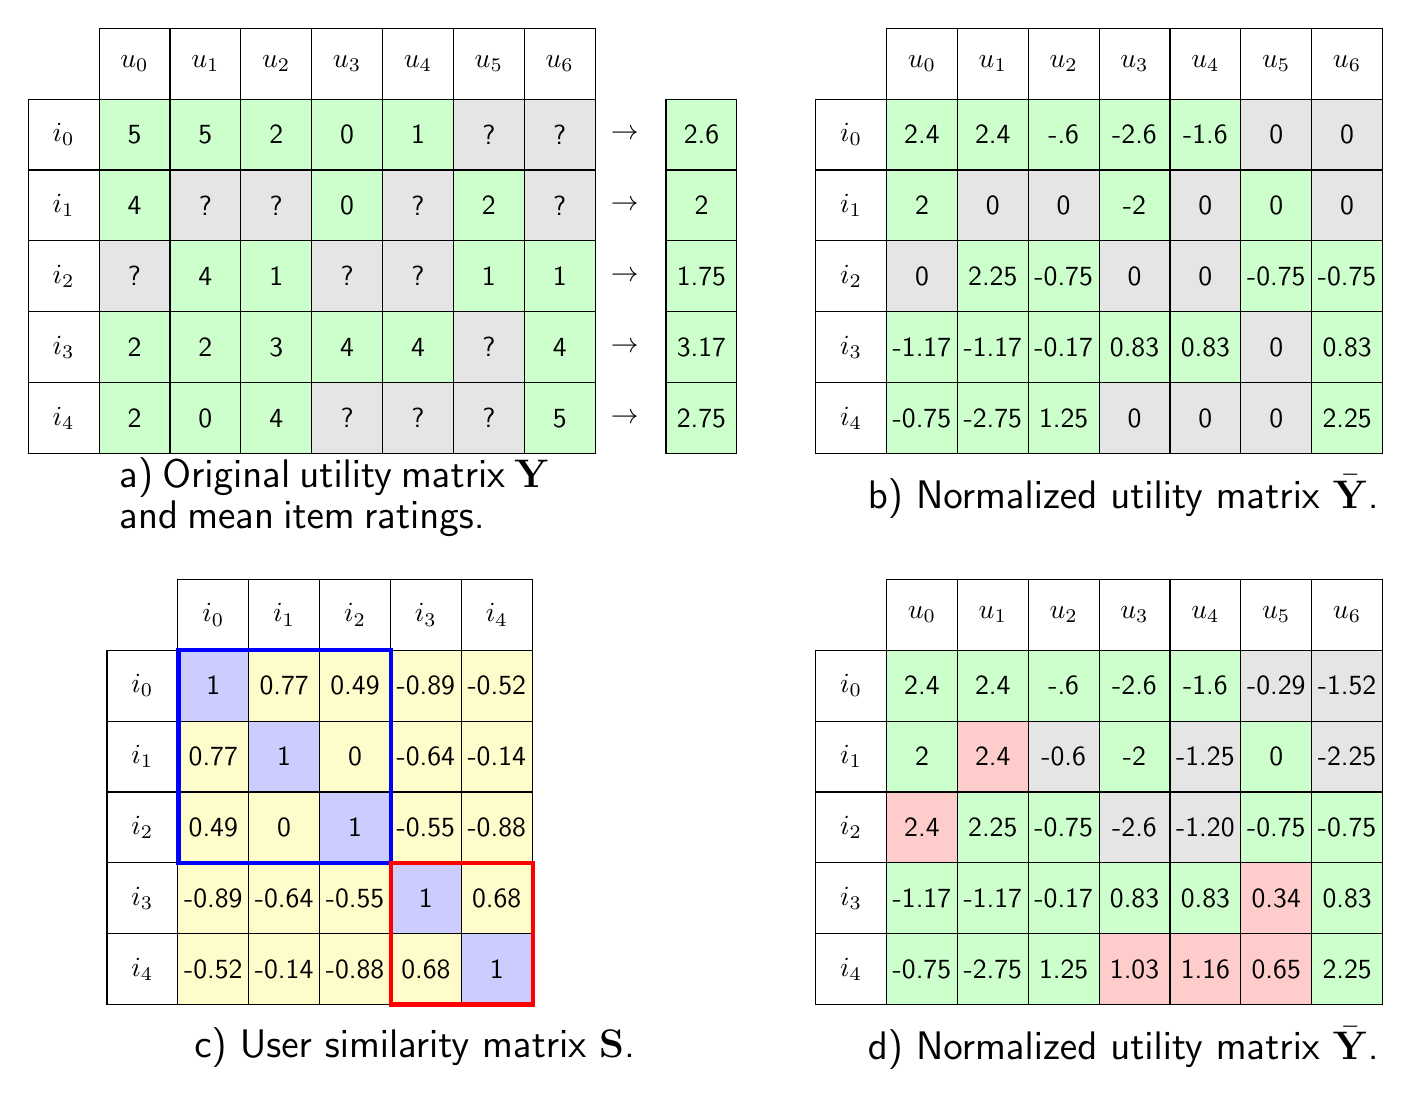
\begin{tikzpicture}
    \begin{scope}
        % \nb{4}{8.25}{white}{\Large a) Original rating matrix $\mathbf{Y}$};

        \node [text width = 5.5cm] at (3, -5.5) {\Large a) Original utility matrix $\mathbf{Y}$ and mean item ratings.};

        \nb{7.75}{1}{white}{$\rightarrow$};
        \nb{7.75}{2}{white}{$\rightarrow$};
        \nb{7.75}{3}{white}{$\rightarrow$};
        \nb{7.75}{4}{white}{$\rightarrow$};
        \nb{7.75}{5}{white}{$\rightarrow$};


        \nn{1}{0}{white}{${u}_0$};
        \nn{1}{1}{green}{5};
        \nn{1}{2}{green}{4};
        \nn{1}{3}{gray}{?};
        \nn{1}{4}{green}{2};
        \nn{1}{5}{green}{2};

        \nn{2}{0}{white}{${u}_1$};
        \nn{2}{1}{green}{5};
        \nn{2}{2}{gray}{?};
        \nn{2}{3}{green}{4};
        \nn{2}{4}{green}{2};
        \nn{2}{5}{green}{0};

        \nn{3}{0}{white}{${u}_2$};
        \nn{3}{1}{green}{2};
        \nn{3}{2}{gray}{?};
        \nn{3}{3}{green}{1};
        \nn{3}{4}{green}{3};
        \nn{3}{5}{green}{4};

        \nn{4}{0}{white}{${u}_3$};
        \nn{4}{1}{green}{0};
        \nn{4}{2}{green}{0};
        \nn{4}{3}{gray}{?};
        \nn{4}{4}{green}{4};
        \nn{4}{5}{gray}{?};

        \nn{5}{0}{white}{${u}_4$};
        \nn{5}{1}{green}{1};
        \nn{5}{2}{gray}{?};
        \nn{5}{3}{gray}{?};
        \nn{5}{4}{green}{4};
        \nn{5}{5}{gray}{?};

        \nn{6}{0}{white}{${u}_5$};
        \nn{6}{1}{gray}{?};
        \nn{6}{2}{green}{2};
        \nn{6}{3}{green}{1};
        \nn{6}{4}{gray}{?};
        \nn{6}{5}{gray}{?};

        \nn{7}{0}{white}{${u}_6$};
        \nn{7}{1}{gray}{?};
        \nn{7}{2}{gray}{?};
        \nn{7}{3}{green}{1};
        \nn{7}{4}{green}{4};
        \nn{7}{5}{green}{5};



        \nnn{0}{1}{white}{${i}_0$};
        \nnn{0}{2}{white}{${i}_1$};
        \nnn{0}{3}{white}{${i}_2$};
        \nnn{0}{4}{white}{${i}_3$};
        \nnn{0}{5}{white}{${i}_4$};

        % \nb{0}{7}{white}{$\bar{u}_j$};
        % \node at (9, -6.3) {$\bar{i}_j$};

        \nn{9}{1}{green}{2.6};
        \nn{9}{2}{green}{2};
        \nn{9}{3}{green}{1.75};
        \nn{9}{4}{green}{3.17};
        \nn{9}{5}{green}{2.75};
        % \nn{9}{6}{green}{3.25};
        % \nn{2}{7}{green}{2.75};
        % \nn{3}{7}{green}{2.5};
        % \nn{4}{7}{green}{1.33};
        % \nn{5}{7}{green}{2.5};
        % \nn{6}{7}{green}{1.5};
        % \nn{7}{7}{green}{3.33};

    \end{scope}



    \begin{scope}[xshift = 10cm]
        % \nb{4}{8.25}{white}{\Large b) $\bar{\mathbf{Y}}$};
        \node  at (3, -5.5) {\Large b) Normalized utility matrix $\bar{\mathbf{Y}}$.};

        \nn{1}{0}{white}{${u}_0$};
        \nn{1}{1}{green}{2.4};
        \nn{1}{2}{green}{2};
        \nn{1}{3}{gray}{0};
        \nn{1}{4}{green}{-1.17};
        \nn{1}{5}{green}{-0.75};

        \nn{2}{0}{white}{${u}_1$};
        \nn{2}{1}{green}{2.4};
        \nn{2}{2}{gray}{0};
        \nn{2}{3}{green}{2.25};
        \nn{2}{4}{green}{-1.17};
        \nn{2}{5}{green}{-2.75};

        \nn{3}{0}{white}{${u}_2$};
        \nn{3}{1}{green}{-.6};
        \nn{3}{2}{gray}{0};
        \nn{3}{3}{green}{-0.75};
        \nn{3}{4}{green}{-0.17};
        \nn{3}{5}{green}{1.25};

        \nn{4}{0}{white}{${u}_3$};
        \nn{4}{1}{green}{-2.6};
        \nn{4}{2}{green}{-2};
        \nn{4}{3}{gray}{0};
        \nn{4}{4}{green}{0.83};
        \nn{4}{5}{gray}{0};

        \nn{5}{0}{white}{${u}_4$};
        \nn{5}{1}{green}{-1.6};
        \nn{5}{2}{gray}{0};
        \nn{5}{3}{gray}{0};
        \nn{5}{4}{green}{0.83};
        \nn{5}{5}{gray}{0};

        \nn{6}{0}{white}{${u}_5$};
        \nn{6}{1}{gray}{0};
        \nn{6}{2}{green}{0};
        \nn{6}{3}{green}{-0.75};
        \nn{6}{4}{gray}{0};
        \nn{6}{5}{gray}{0};

        \nn{7}{0}{white}{${u}_6$};
        \nn{7}{1}{gray}{0};
        \nn{7}{2}{gray}{0};
        \nn{7}{3}{green}{-0.75};
        \nn{7}{4}{green}{0.83};
        \nn{7}{5}{green}{2.25};



        \nnn{0}{1}{white}{${i}_0$};
        \nnn{0}{2}{white}{${i}_1$};
        \nnn{0}{3}{white}{${i}_2$};
        \nnn{0}{4}{white}{${i}_3$};
        \nnn{0}{5}{white}{${i}_4$};

    \end{scope}
    

    \begin{scope}[xshift = 1cm, yshift = -7cm]
        % \nb{4}{8.25}{white}{\Large c) ${{S}}$};
        \node  at (3, -5.5) {\Large c) User similarity matrix ${\mathbf{S}}$.};

        \nn{1}{0}{white}{${i}_0$};
        \nn{1}{1}{blue}{1};
        \nn{1}{2}{yellow}{0.77};
        \nn{1}{3}{yellow}{0.49};
        \nn{1}{4}{yellow}{-0.89};
        \nn{1}{5}{yellow}{-0.52};

        \nn{2}{0}{white}{${i}_1$};
        \nn{2}{1}{yellow}{0.77};
        \nn{2}{2}{blue}{1};
        \nn{2}{3}{yellow}{0};
        \nn{2}{4}{yellow}{-0.64};
        \nn{2}{5}{yellow}{-0.14};

        \nn{3}{0}{white}{${i}_2$};
        \nn{3}{1}{yellow}{0.49};
        \nn{3}{2}{yellow}{0};
        \nn{3}{3}{blue}{1};
        \nn{3}{4}{yellow}{-0.55};
        \nn{3}{5}{yellow}{-0.88};

        \nn{4}{0}{white}{${i}_3$};
        \nn{4}{1}{yellow}{-0.89};
        \nn{4}{2}{yellow}{-0.64};
        \nn{4}{3}{yellow}{-0.55};
        \nn{4}{4}{blue}{1};
        \nn{4}{5}{yellow}{0.68};

        \nn{5}{0}{white}{${i}_4$};
        \nn{5}{1}{yellow}{-0.52};
        \nn{5}{2}{yellow}{-0.14};
        \nn{5}{3}{yellow}{-0.88};
        \nn{5}{4}{yellow}{0.68};
        \nn{5}{5}{blue}{1};

      

        \nnn{0}{1}{white}{${i}_0$};
        \nnn{0}{2}{white}{${i}_1$};
        \nnn{0}{3}{white}{${i}_2$};
        \nnn{0}{4}{white}{${i}_3$};
        \nnn{0}{5}{white}{${i}_4$};
        % \nnn{0}{6}{white}{${u}_5$};
        % \nnn{0}{7}{white}{${u}_6$};
        \draw [ultra thick, draw = blue] (0*\d, 0.5*\q) rectangle(3*\d, 3.5*\q);
        \draw [ultra thick, draw = red] (3*\d, 3.5*\q) rectangle(5*\d, 5.5*\q);
    \end{scope}

        \begin{scope}[xshift = 10cm, yshift = -7cm]
        % \nb{4}{8.25}{white}{\Large b) $\bar{\mathbf{Y}}$};
        \node  at (3, -5.5) {\Large d) Normalized utility matrix $\bar{\mathbf{Y}}$.};

        \nn{1}{0}{white}{${u}_0$};
        \nn{1}{1}{green}{2.4};
        \nn{1}{2}{green}{2};
        \nn{1}{3}{red}{2.4};
        \nn{1}{4}{green}{-1.17};
        \nn{1}{5}{green}{-0.75};

        \nn{2}{0}{white}{${u}_1$};
        \nn{2}{1}{green}{2.4};
        \nn{2}{2}{red}{2.4};
        \nn{2}{3}{green}{2.25};
        \nn{2}{4}{green}{-1.17};
        \nn{2}{5}{green}{-2.75};

        \nn{3}{0}{white}{${u}_2$};
        \nn{3}{1}{green}{-.6};
        \nn{3}{2}{gray}{-0.6};
        \nn{3}{3}{green}{-0.75};
        \nn{3}{4}{green}{-0.17};
        \nn{3}{5}{green}{1.25};

        \nn{4}{0}{white}{${u}_3$};
        \nn{4}{1}{green}{-2.6};
        \nn{4}{2}{green}{-2};
        \nn{4}{3}{gray}{-2.6};
        \nn{4}{4}{green}{0.83};
        \nn{4}{5}{red}{1.03};

        \nn{5}{0}{white}{${u}_4$};
        \nn{5}{1}{green}{-1.6};
        \nn{5}{2}{gray}{-1.25};
        \nn{5}{3}{gray}{-1.20};
        \nn{5}{4}{green}{0.83};
        \nn{5}{5}{red}{1.16};

        \nn{6}{0}{white}{${u}_5$};
        \nn{6}{1}{gray}{-0.29};
        \nn{6}{2}{green}{0};
        \nn{6}{3}{green}{-0.75};
        \nn{6}{4}{red}{0.34};
        \nn{6}{5}{red}{0.65};

        \nn{7}{0}{white}{${u}_6$};
        \nn{7}{1}{gray}{-1.52};
        \nn{7}{2}{gray}{-2.25};
        \nn{7}{3}{green}{-0.75};
        \nn{7}{4}{green}{0.83};
        \nn{7}{5}{green}{2.25};



        \nnn{0}{1}{white}{${i}_0$};
        \nnn{0}{2}{white}{${i}_1$};
        \nnn{0}{3}{white}{${i}_2$};
        \nnn{0}{4}{white}{${i}_3$};
        \nnn{0}{5}{white}{${i}_4$};

    \end{scope}
    
    % %%%%%%%%%%%%%%%%%%%%
    % \begin{scope}[xshift = 0cm, yshift = -9cm]
    %     % \nb{4}{6.25}{white}{\Large d) $\hat{\mathbf{Y}}$};
    %     \node  at (3, -5.75) {\Large d) $\hat{\mathbf{Y}}$};

    %     \nn{1}{0}{white}{${u}_0$};
    %             \nn{1}{1}{green}{1.75};
    %             \nn{1}{2}{green}{0.75};
    %             \nn{1}{3}{red}{0.91};
    %             \nn{1}{4}{green}{-1.25};
    %             \nn{1}{5}{green}{-1.25};

    %             \nn{2}{0}{white}{${u}_1$};
    %             \nn{2}{1}{green}{2.25};
    %             % \nn{2}{2}{red}{0.48};
    %             \begin{scope}[xshift = 2*\d cm, yshift = 2*\q cm]
    %                 \node at (0, 0) [anchor = east, draw = blue, ultra thick, inner sep = 0, fill = red!20, minimum height = .9cm, minimum width = .9cm] {\color{blue}{0.48}};
    %             \end{scope}

    %             \nn{2}{3}{green}{1.25};
    %             \nn{2}{4}{green}{-0.75};
    %             \nn{2}{5}{green}{-2.75};

    %             \nn{3}{0}{white}{${u}_2$};
    %             \nn{3}{1}{green}{-0.5};
    %             \nn{3}{2}{gray}{-0.17};
    %             \nn{3}{3}{green}{-1.5};
    %             \nn{3}{4}{green}{0.5};
    %             \nn{3}{5}{green}{1.5};

    %             \nn{4}{0}{white}{${u}_3$};
    %             \nn{4}{1}{green}{-1.33};
    %             \nn{4}{2}{green}{-1.33};
    %             \nn{4}{3}{gray}{-1.84};
    %             \nn{4}{4}{green}{2.67};
    %             \nn{4}{5}{red}{1.57};

    %             \nn{5}{0}{white}{${u}_4$};
    %             \nn{5}{1}{green}{-1.5};
    %             \nn{5}{2}{gray}{-1.33};
    %             \nn{5}{3}{gray}{-1.78};
    %             \nn{5}{4}{green}{1.5};
    %             \nn{5}{5}{red}{1.56};

    %             \nn{6}{0}{white}{${u}_5$};
    %             \nn{6}{1}{red}{0.18};
    %             \nn{6}{2}{green}{0.5};
    %             \nn{6}{3}{green}{-0.5};
    %             \nn{6}{4}{red}{0.59};
    %             \nn{6}{5}{red}{1.59};

    %             \nn{7}{0}{white}{${u}_6$};
    %             \nn{7}{1}{gray}{-0.63};
    %             \nn{7}{2}{red}{0.05};
    %             \nn{7}{3}{green}{-2.33};
    %             \nn{7}{4}{green}{0.67};
    %             \nn{7}{5}{green}{1.67};



    %             \nnn{0}{1}{white}{${i}_0$};
    %             \nnn{0}{2}{white}{${i}_1$};
    %             \nnn{0}{3}{white}{${i}_2$};
    %             \nnn{0}{4}{white}{${i}_3$};
    %             \nnn{0}{5}{white}{${i}_4$};

    %     % \nb{-.5}{7}{white}{$\|{u}_j\|_2^2$};

    %     % \nn{1}{7}{green}{6};
    %     % \nn{2}{7}{green}{59/4};
    %     % \nn{3}{7}{green}{5};
    %     % \nn{4}{7}{green}{32/3};
    %     % \nn{5}{7}{green}{9/2};
    %     % \nn{6}{7}{green}{2};
    %     % \nn{7}{7}{green}{14/3};
    % \end{scope}

    % \def\l{-.8} % linespace
    % \begin{scope}[xshift = 7cm, yshift = -9cm]
    %     \node  at (3, -5.75) {\Large e) Example};

    %     \node at (0, 0) [anchor = west, align = left, scale = 1.2] {Predict normalized rating of $u_1$ on $i_1$ with $k=2$};
    %     \node at (0, \l) [anchor = west, align = left, scale = 1.2] {Users who rated $i_1$ : \{$u_0, u_3, u_5$\} };
    %     \node at (0, 2*\l) [anchor = west, align = left, scale = 1.2] {Corresponding similarities $i_1$ : \{0.83, -0.40, -0.23\} };
    %     \node at (0, 3*\l) [anchor = west, align = left, scale = 1.2] {$\Rightarrow$ most similar users: $\mathcal{N}(u_1, i_1) = $\{$u_0, u_5$\} };
    %     \node at (0, 4*\l) [anchor = west, align = left, scale = 1.2] {with \bf{normalized} ratings \{0.75, 0.5\}};
    %     \node at (0, 5.5*\l) [anchor = west, align = left, scale = 1.5] {$\Rightarrow$ $\hat{y}_{i_1, u_1} = \frac{0.83*0.75 + (-0.23)*0.5}{0.83 + |-0.23|} \approx \color{blue}{0.48}$};
        
    % \end{scope}

    % \begin{scope}[xshift = 18cm, yshift = -9cm]
    %     % \nb{4}{6.25}{white}{\Large e) Full ${\mathbf{Y}}$};
    %     \node  at (3, -5.75) {\Large f) Full ${\mathbf{Y}}$};

    %     \nn{1}{0}{white}{${u}_0$};
    %     \nn{1}{1}{green}{5};
    %     \nn{1}{2}{green}{4};
    %     \nn{1}{3}{gray}{4.15};
    %     \nn{1}{4}{green}{2};
    %     \nn{1}{5}{green}{2};

    %     \nn{2}{0}{white}{${u}_1$};
    %     \nn{2}{1}{green}{5};
    %     \nn{2}{2}{gray}{3.23};
    %     \nn{2}{3}{green}{4};
    %     \nn{2}{4}{green}{2};
    %     \nn{2}{5}{green}{0};

    %     \nn{3}{0}{white}{${u}_2$};
    %     \nn{3}{1}{green}{2};
    %     \nn{3}{2}{gray}{2.33};
    %     \nn{3}{3}{green}{1};
    %     \nn{3}{4}{green}{3};
    %     \nn{3}{5}{green}{4};

    %     \nn{4}{0}{white}{${u}_3$};
    %     \nn{4}{1}{green}{0};
    %     \nn{4}{2}{green}{0};
    %     \nn{4}{3}{gray}{-0.5};
    %     \nn{4}{4}{green}{4};
    %     \nn{4}{5}{gray}{2.9};

    %     \nn{5}{0}{white}{${u}_4$};
    %     \nn{5}{1}{green}{1};
    %     \nn{5}{2}{gray}{1.67};
    %     \nn{5}{3}{gray}{0.71};
    %     \nn{5}{4}{green}{4};
    %     \nn{5}{5}{gray}{4.06};

    %     \nn{6}{0}{white}{${u}_5$};
    %     \nn{6}{1}{gray}{1.68};
    %     \nn{6}{2}{green}{2};
    %     \nn{6}{3}{green}{1};
    %     \nn{6}{4}{gray}{2.10};
    %     \nn{6}{5}{gray}{3.10};

    %     \nn{7}{0}{white}{${u}_6$};
    %     \nn{7}{1}{gray}{2.70};
    %     \nn{7}{2}{gray}{3.38};
    %     \nn{7}{3}{green}{1};
    %     \nn{7}{4}{green}{4};
    %     \nn{7}{5}{green}{5};



    %     \nnn{0}{1}{white}{${i}_0$};
    %     \nnn{0}{2}{white}{${i}_1$};
    %     \nnn{0}{3}{white}{${i}_2$};
    %     \nnn{0}{4}{white}{${i}_3$};
    %     \nnn{0}{5}{white}{${i}_4$};

    % \end{scope}
\end{tikzpicture}
\end{document}